\documentclass[12pt,a4paper]{article}

\usepackage[utf8]{inputenc}
\usepackage{graphicx}
\usepackage{hyperref}
\usepackage{geometry}
\usepackage{xcolor}
\usepackage{listings}
\usepackage{booktabs}
\usepackage{float}
\usepackage{titlesec}
\usepackage{tcolorbox}
\usepackage{tabularx}

\geometry{margin=1in}

% Colors for code blocks
\definecolor{codebg}{rgb}{0.95,0.95,0.95}
\definecolor{codecomment}{rgb}{0.4,0.4,0.4}
\definecolor{codekeyword}{rgb}{0.0,0.4,0.8}
\definecolor{codestring}{rgb}{0.6,0.1,0.1}

\lstset{
    backgroundcolor=\color{codebg},
    basicstyle=\ttfamily\footnotesize,
    commentstyle=\color{codecomment},
    keywordstyle=\color{codekeyword},
    stringstyle=\color{codestring},
    breaklines=true,
    captionpos=b,
    frame=single,
    rulecolor=\color{lightgray},
    numbers=left,
    numberstyle=\tiny\color{gray},
    showstringspaces=false
}

\title{
    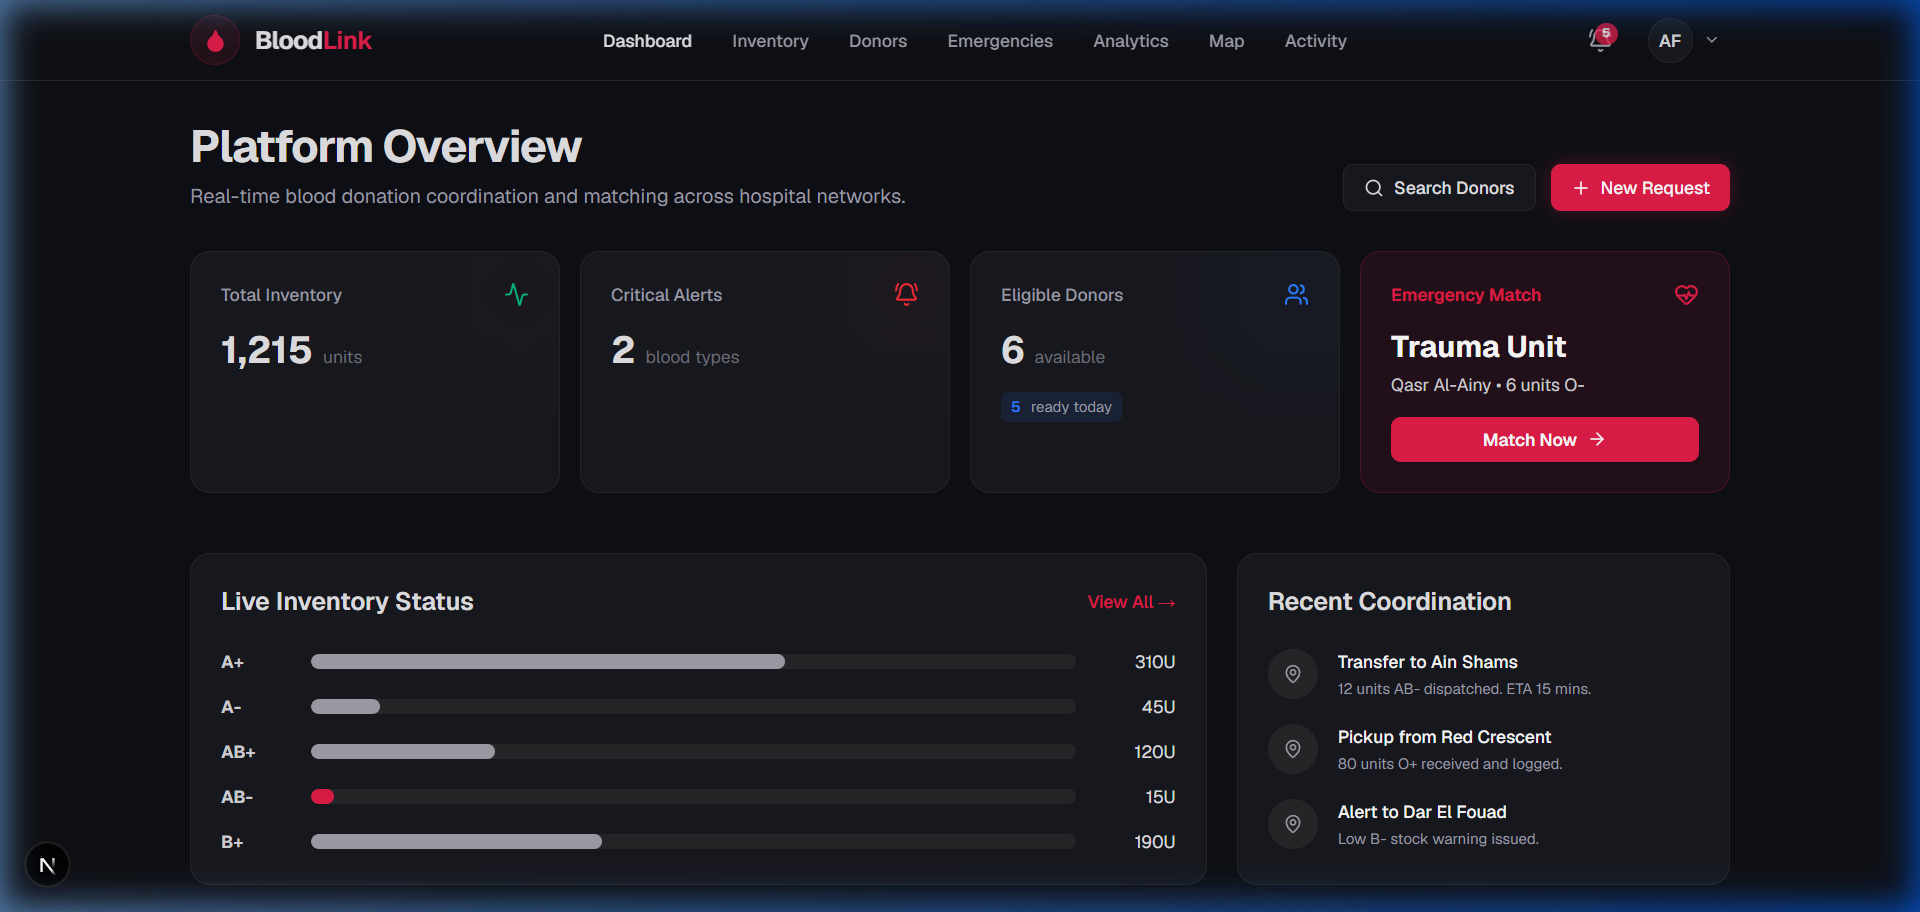
\includegraphics[width=0.2\textwidth]{figures/dashboard.png} \\ % Using dashboard as a placeholder logo if needed, or just remove
    \vspace{1cm}
    \textbf{BloodLink Platform Report} \\
    \large Real-time Blood Bank Management \& Intelligent Donor Matching System
}
\author{Biomedical Engineering Project}
\date{\today}

\begin{document}

\maketitle
\tableofcontents
\newpage

\section{Introduction}
BloodLink is a comprehensive, full-stack clinical platform designed to modernize blood bank management, streamline donor networks, and optimize emergency blood request fulfillment. The system transitions traditional CRUD-based blood management into a professional, production-grade clinical tool by integrating real-time analytics, geospatial tracking, and an intelligent multi-factor matching engine.

\section{System Architecture and Technology Stack}
The platform employs a modern decoupled architecture, ensuring scalability, maintainability, and high performance.

\subsection{Backend Stack}
\begin{itemize}
    \item \textbf{Framework:} NestJS (v11.x) - Provides a robust, modular, and opinionated architecture using TypeScript.
    \item \textbf{Database:} PostgreSQL (v17) - Relational database for robust data integrity.
    \item \textbf{ORM:} TypeORM (v0.3.x) - Object-Relational Mapper for seamless database interactions.
    \item \textbf{Authentication:} Passport + JWT - Secure, stateless token-based authentication.
\end{itemize}

\subsection{Frontend Stack}
\begin{itemize}
    \item \textbf{Framework:} Next.js (v16.2) - React framework utilizing the App Router for server-side rendering and optimized client routing.
    \item \textbf{Styling:} Tailwind CSS - Utility-first CSS framework for a responsive, modern, dark-themed UI.
    \item \textbf{Data Visualization:} Recharts - For rendering dynamic analytics dashboards.
    \item \textbf{Mapping:} Leaflet / React-Leaflet - For interactive GIS-based visualization of donors and hospitals.
\end{itemize}

\section{Core Database Schema}
The database schema is designed to model the complex relationships between users, donors, inventory, and emergency events.

\subsection{Key Entities}
\begin{enumerate}
    \item \textbf{User (\texttt{users}):} Manages staff, admins, managers, and donor logins. Includes role-based access control (RBAC).
    \item \textbf{Donor (\texttt{donors}):} Stores detailed donor profiles including blood type, location (city/district), donation history, reliability score, and current availability status.
    \item \textbf{Blood Inventory (\texttt{blood\_inventory}):} Tracks real-time stock levels of all 8 blood types (O$\pm$, A$\pm$, B$\pm$, AB$\pm$), categorizing them into Healthy, Warning, or Critical states.
    \item \textbf{Emergency Request (\texttt{emergency\_requests}):} Logs critical needs from specific hospital departments, detailing required blood type, urgency level, and units needed.
    \item \textbf{Audit Log (\texttt{audit\_logs}):} A centralized tracking system recording all major CRUD operations, logins, and system events for clinical transparency and compliance.
\end{enumerate}

\begin{figure}[H]
    \centering
    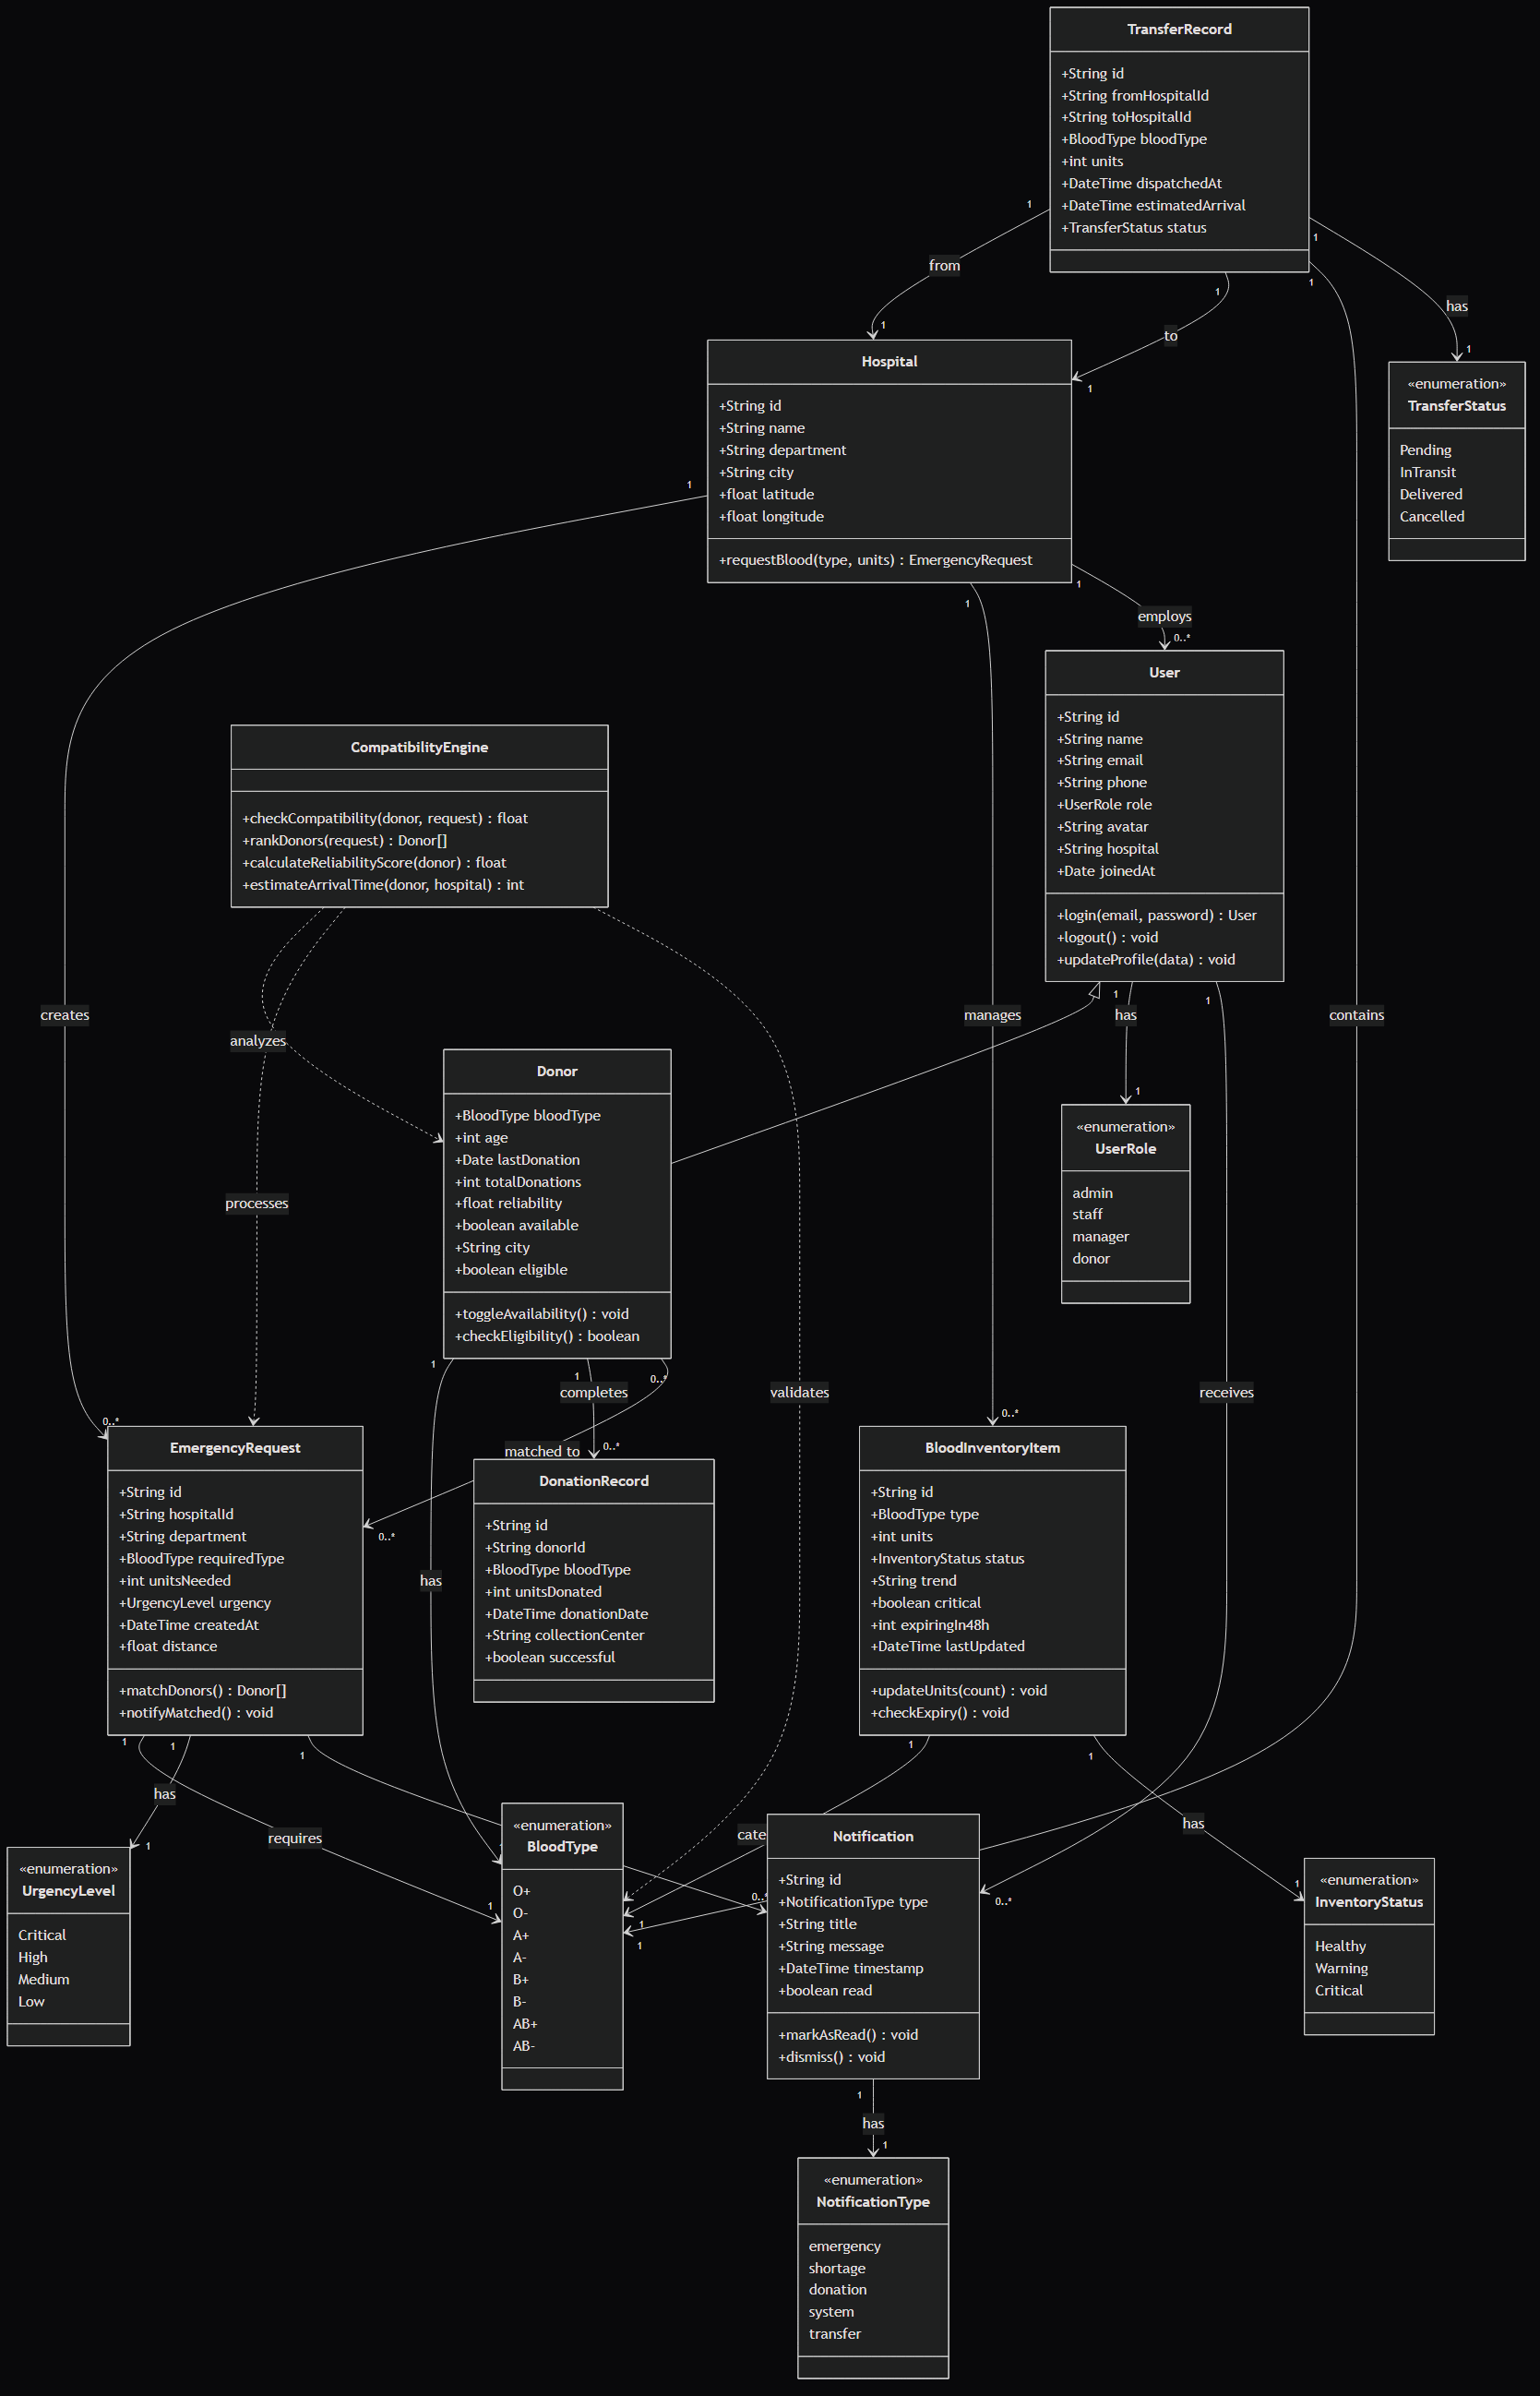
\includegraphics[width=0.9\textwidth]{figures/class_diagram.png}
    \caption{UML Class Diagram illustrating Entity Relationships.}
\end{figure}

\section{Key Features and Modules}

\subsection{Dashboard Overview}
The main dashboard acts as the central hub, displaying high-level metrics such as total inventory units, active critical alerts, available eligible donors, and active emergency matches.

\begin{figure}[H]
    \centering
    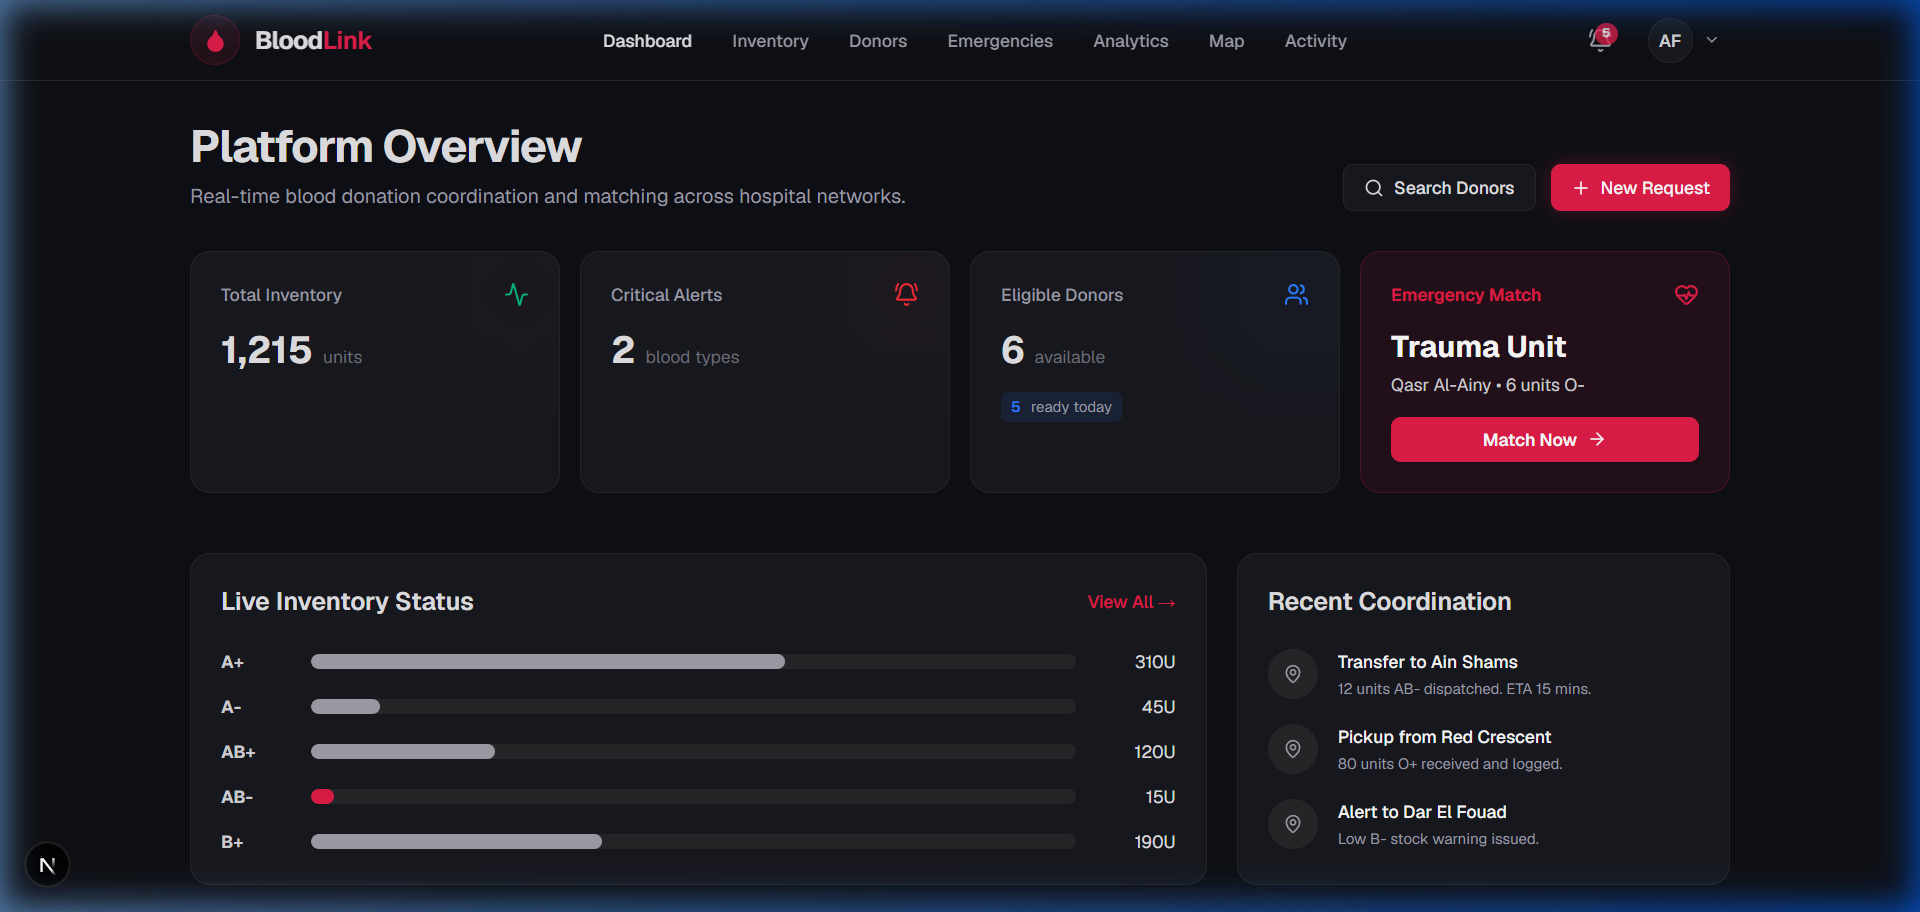
\includegraphics[width=\textwidth]{figures/dashboard.png}
    \caption{BloodLink Dashboard Overview.}
\end{figure}

\subsection{Blood Inventory Management}
The inventory module provides real-time tracking of blood stocks. It automatically calculates status thresholds (Healthy $\ge$ 100, Warning 20--99, Critical $<$ 20 units). It also tracks units expiring within 48 hours to prevent waste.

\begin{figure}[H]
    \centering
    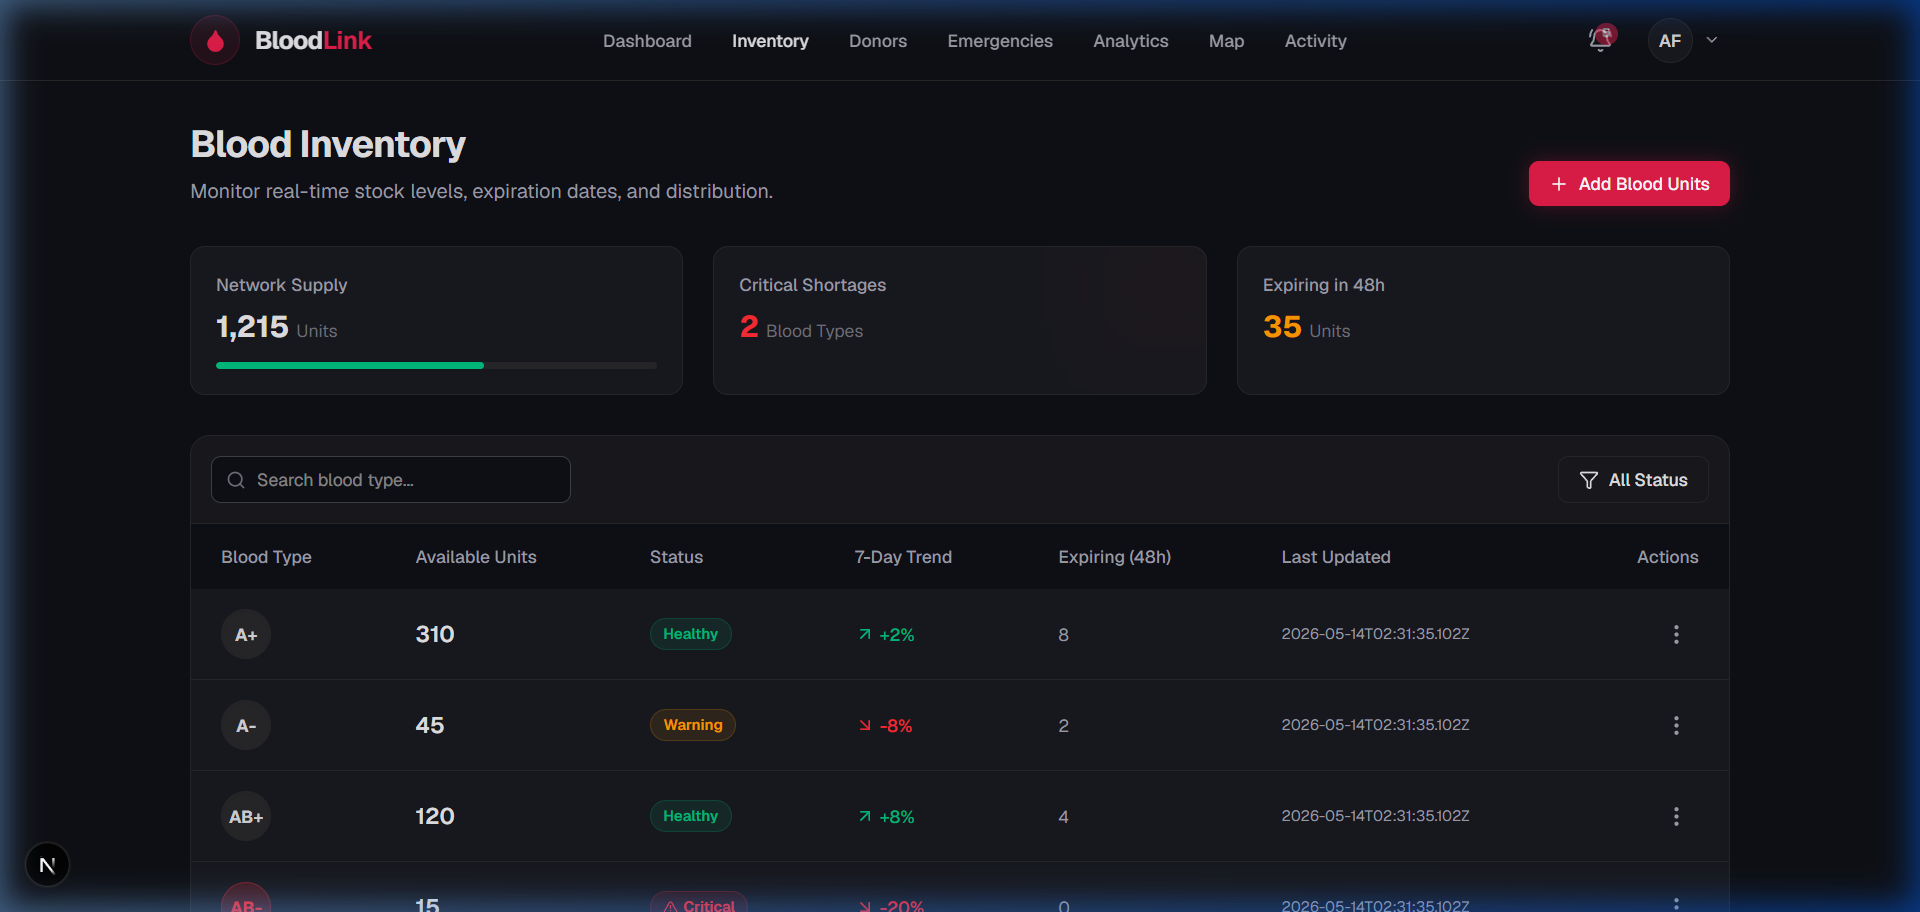
\includegraphics[width=\textwidth]{figures/inventory.png}
    \caption{Live Blood Inventory Tracking.}
\end{figure}

\subsection{Donor Management \& Self-Service Portal}
A comprehensive donor registry allows staff to filter by blood type, availability, and location. Donors also have a dedicated portal where they can view their WHO 56-day eligibility countdown, toggle their availability, and track their donation history.

\begin{figure}[H]
    \centering
    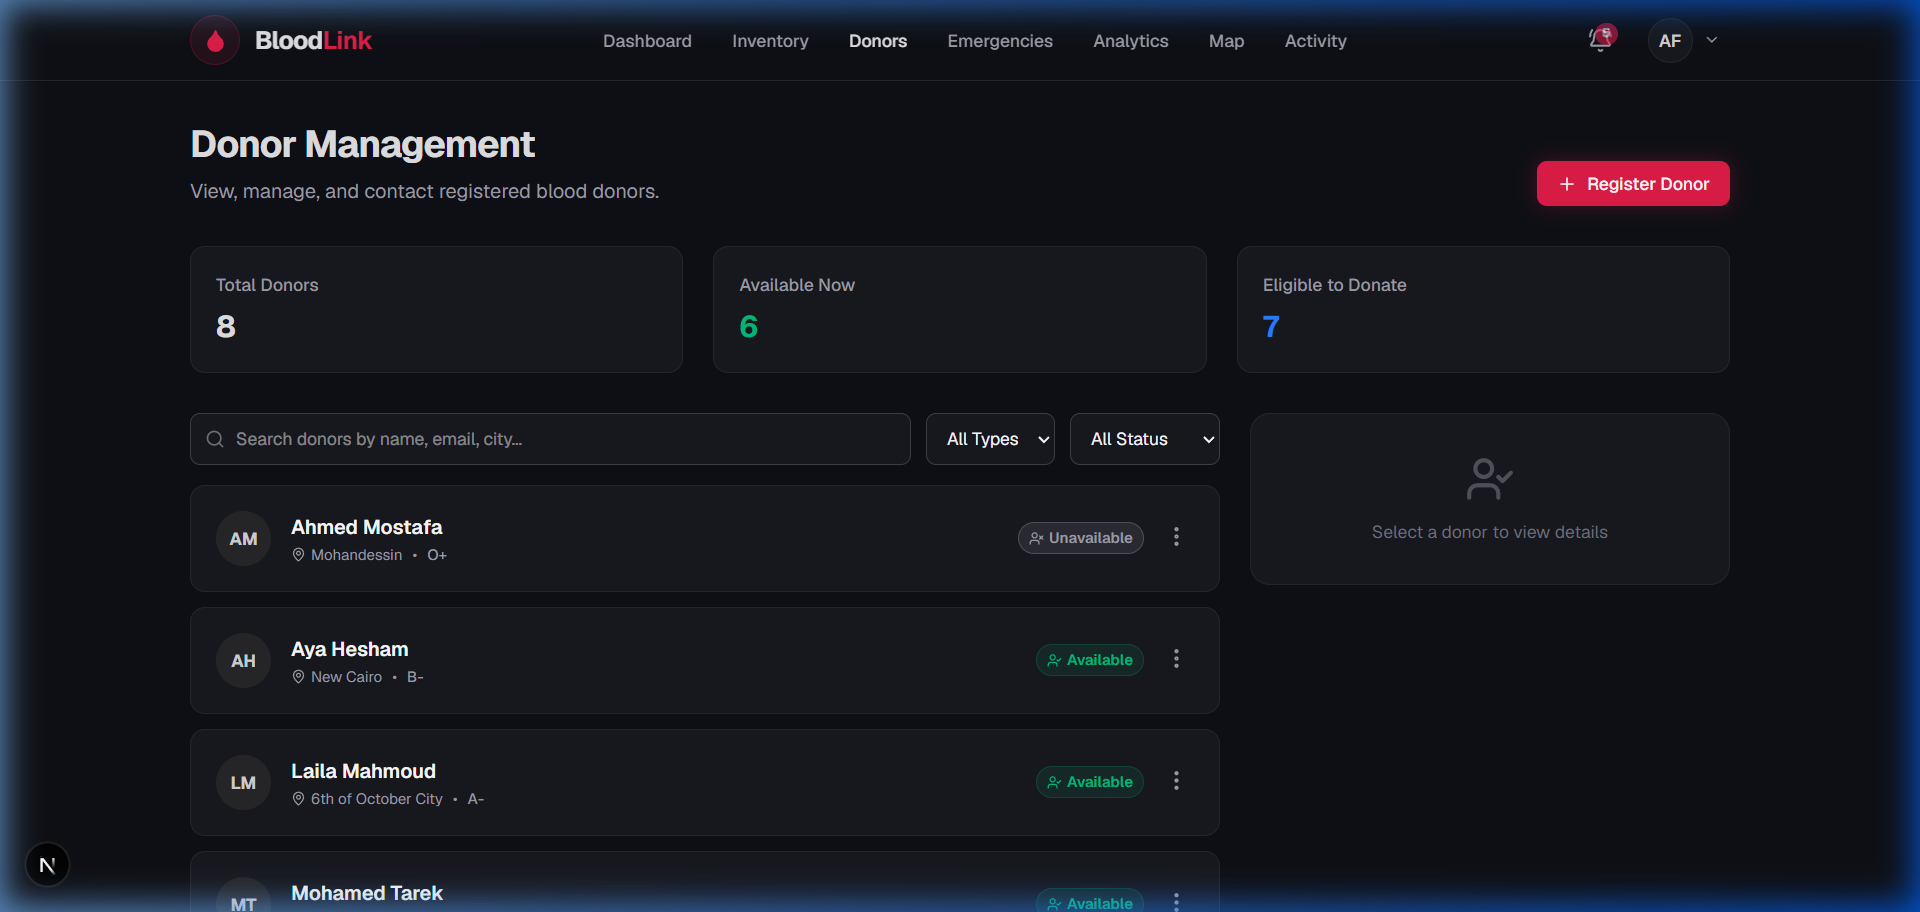
\includegraphics[width=\textwidth]{figures/donors.png}
    \caption{Donor Registry Interface.}
\end{figure}

\subsection{Emergency Request Handling}
Hospitals can broadcast emergency requests specifying the required blood type, units, and urgency level (Critical, High, Medium, Low). This module tightly integrates with the Matching Engine to find donors immediately.

\begin{figure}[H]
    \centering
    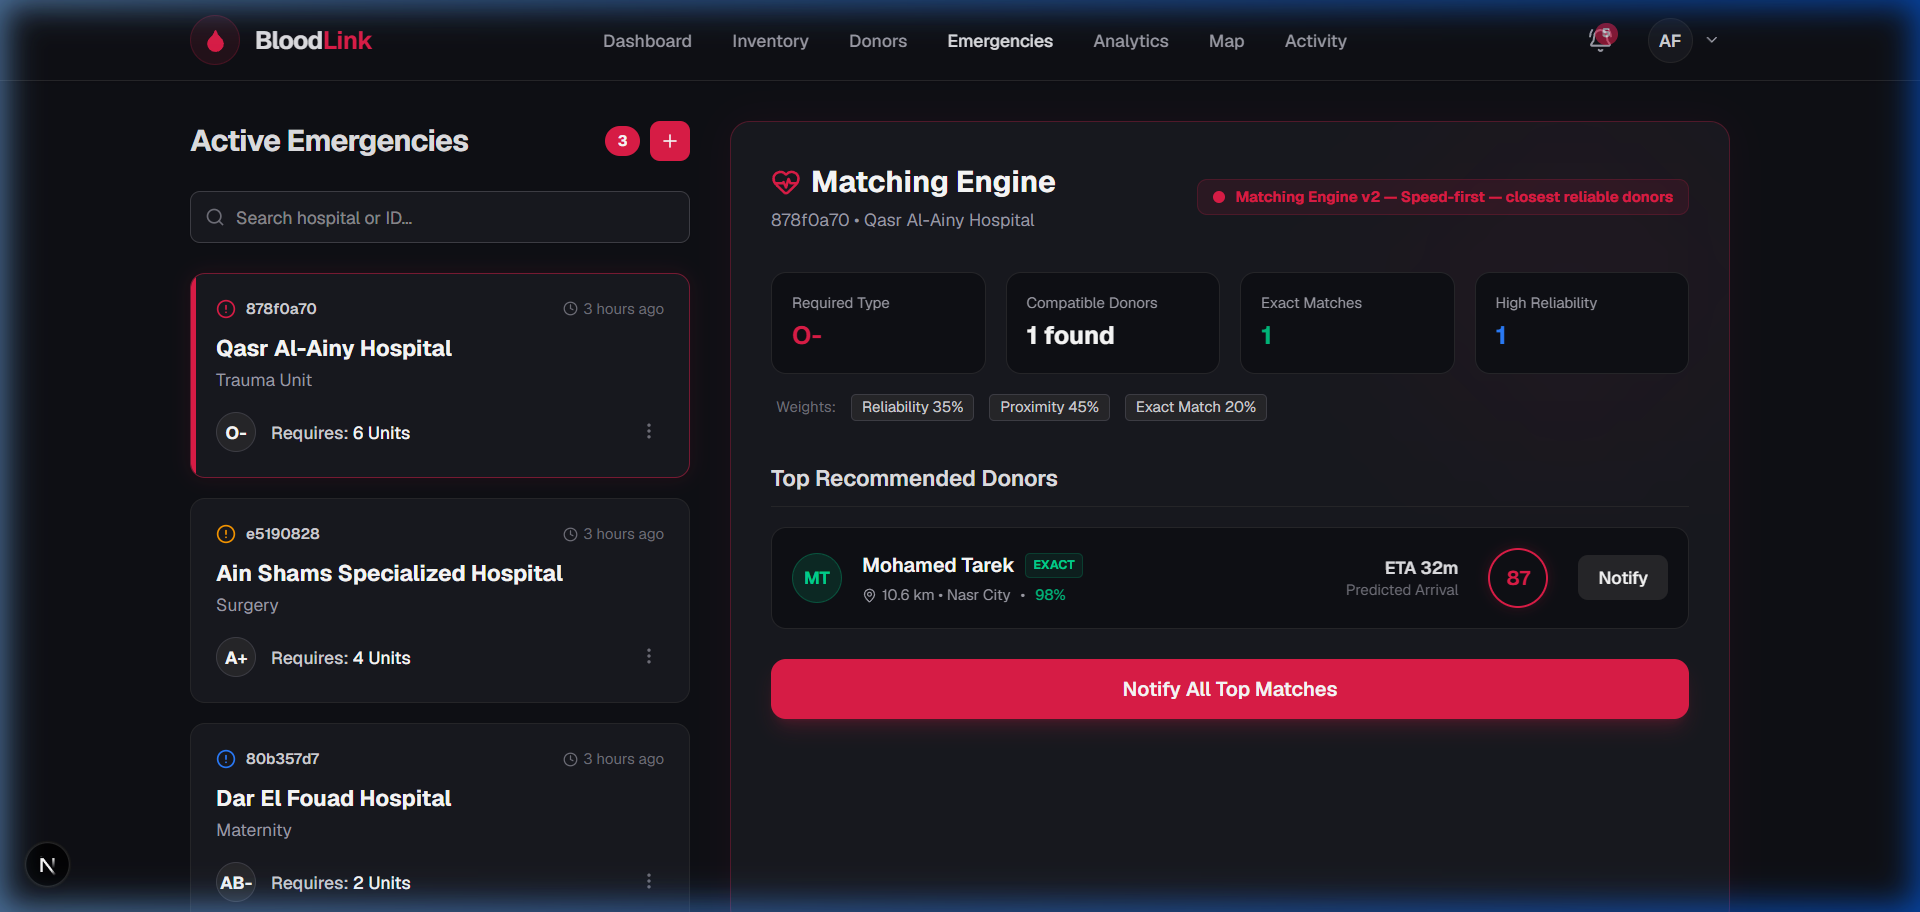
\includegraphics[width=\textwidth]{figures/emergencies.png}
    \caption{Emergency Requests Dashboard.}
\end{figure}

\subsection{Analytics \& Geospatial Mapping}
The analytics module provides deep insights through Recharts, showing blood type distributions, reliability buckets, and inventory health. The map module utilizes Leaflet to visualize the geospatial distribution of donors relative to hospital emergency requests across Cairo districts.

\begin{figure}[H]
    \centering
    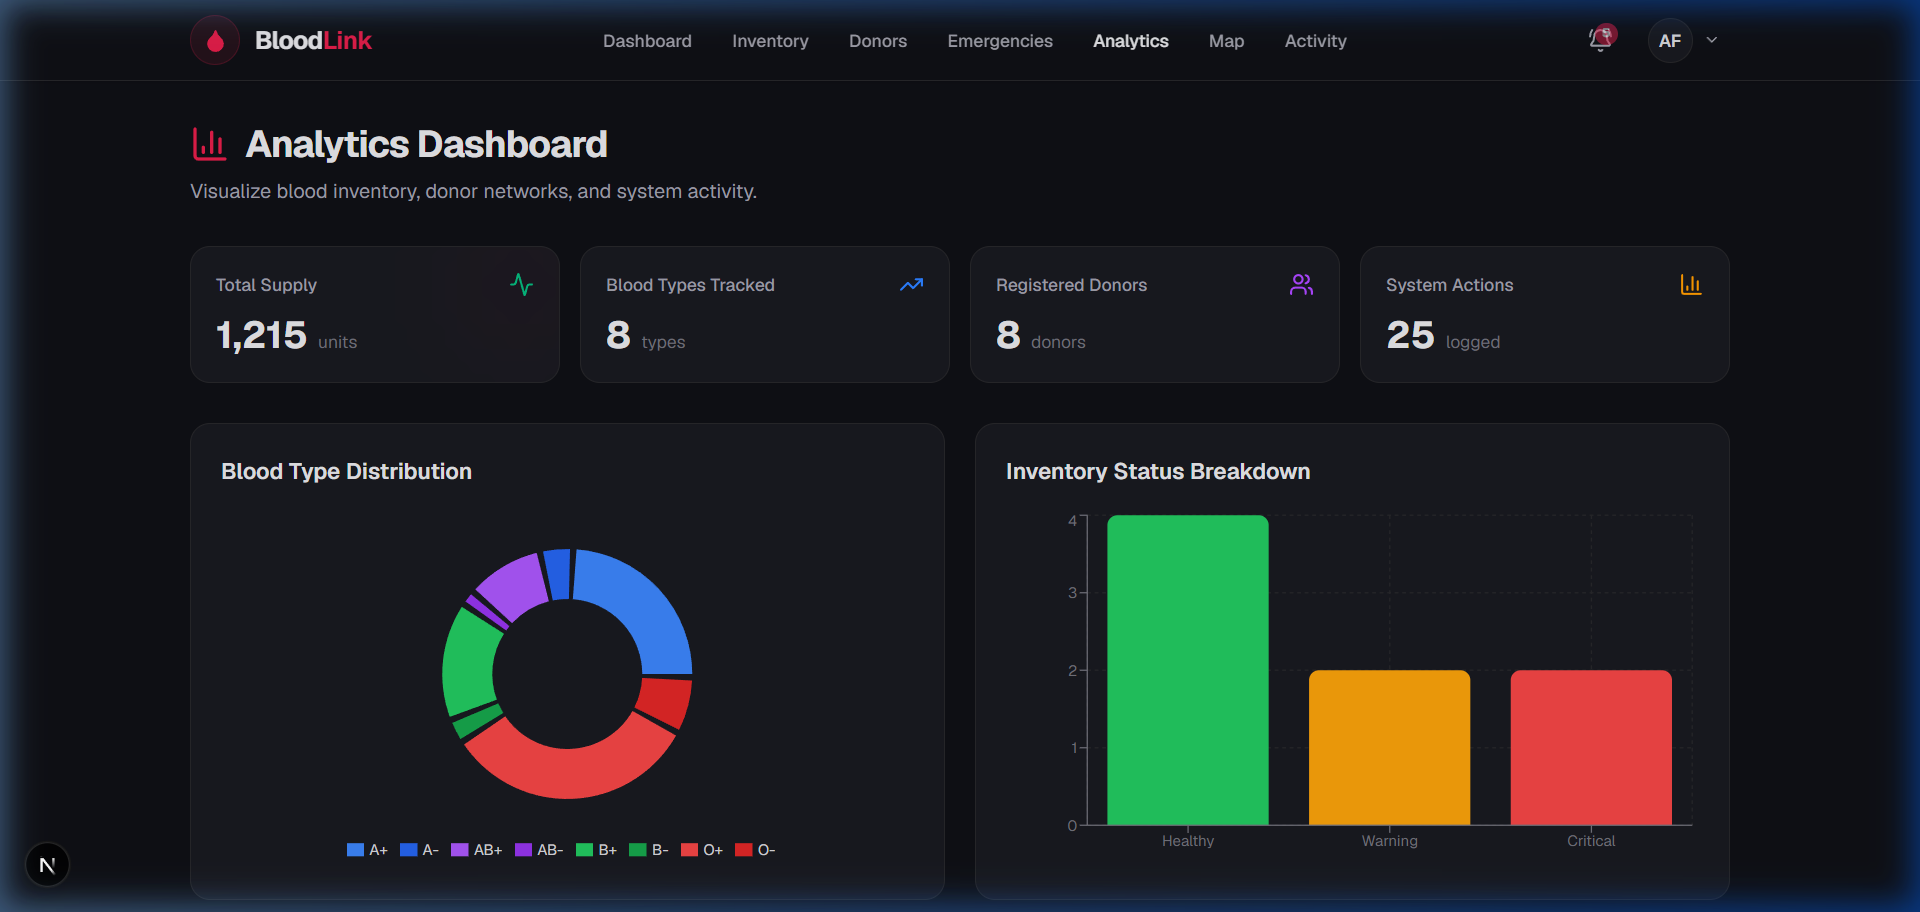
\includegraphics[width=\textwidth]{figures/analytics.png}
    \caption{Interactive Analytics Dashboard.}
\end{figure}

\begin{figure}[H]
    \centering
    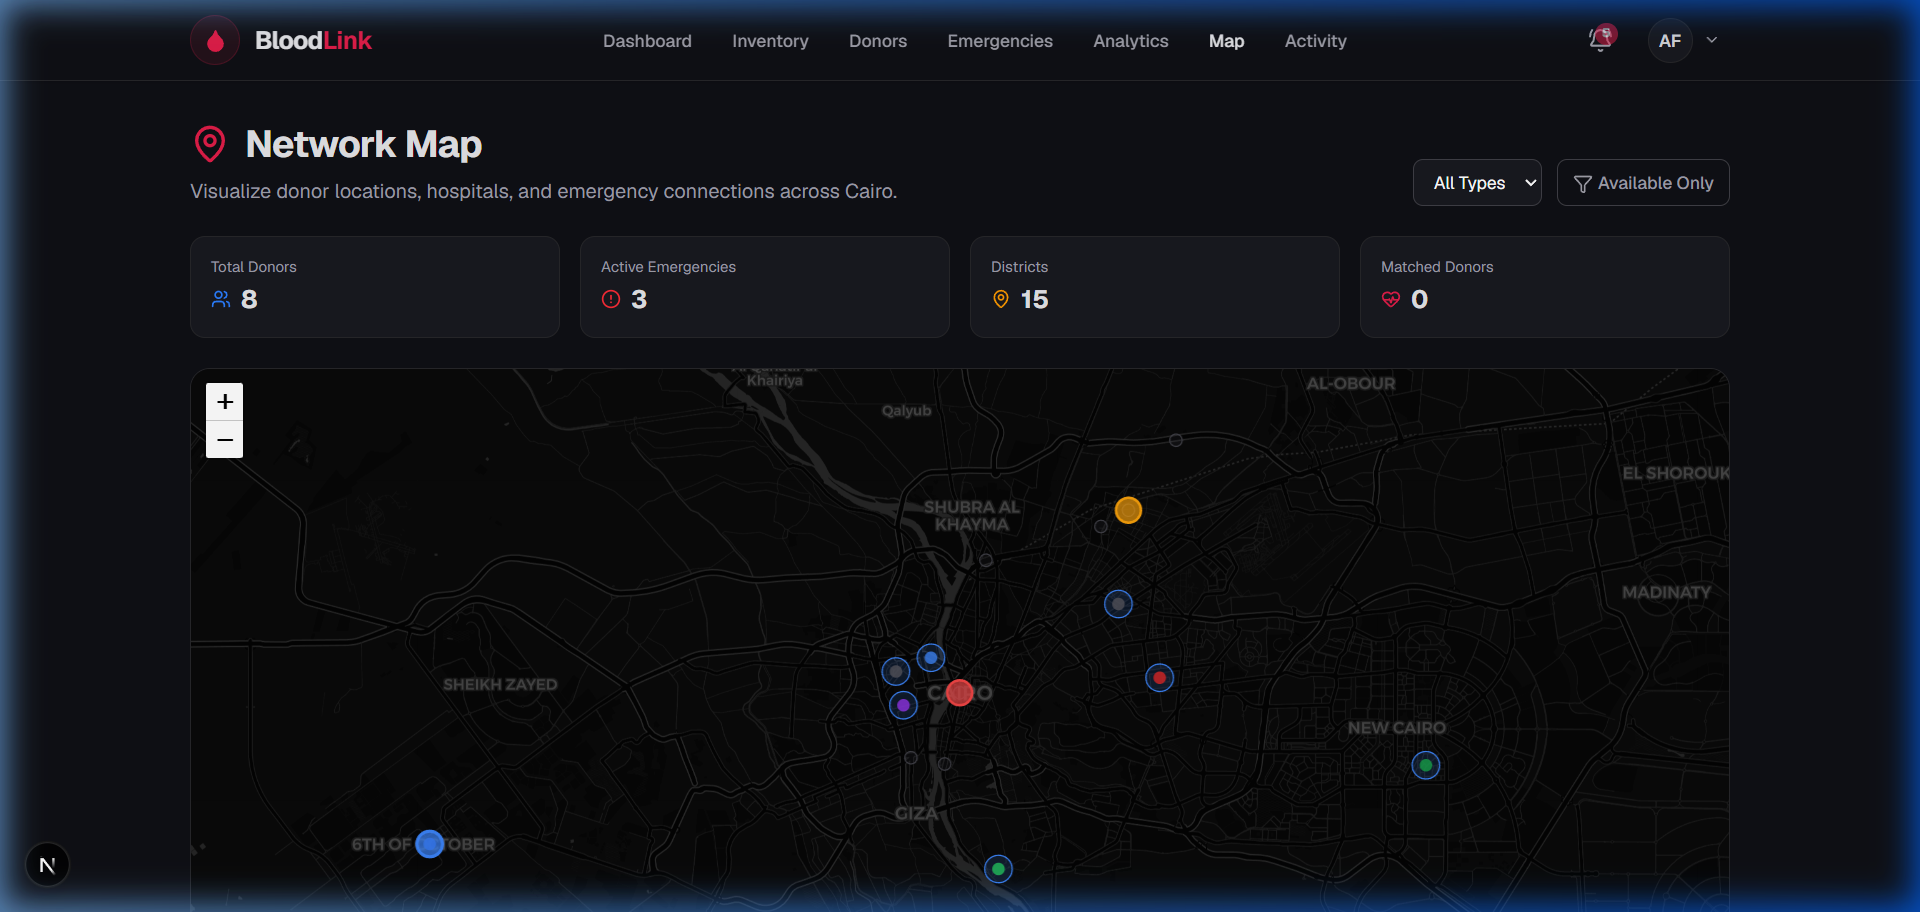
\includegraphics[width=\textwidth]{figures/map.png}
    \caption{Geospatial Map of Cairo Donors and Hospitals.}
\end{figure}

\subsection{Centralized Audit Logging}
To ensure clinical-grade transparency, the \texttt{AuditService} is injected across all core modules. It logs every creation, update, deletion, match run, and login event.

\begin{figure}[H]
    \centering
    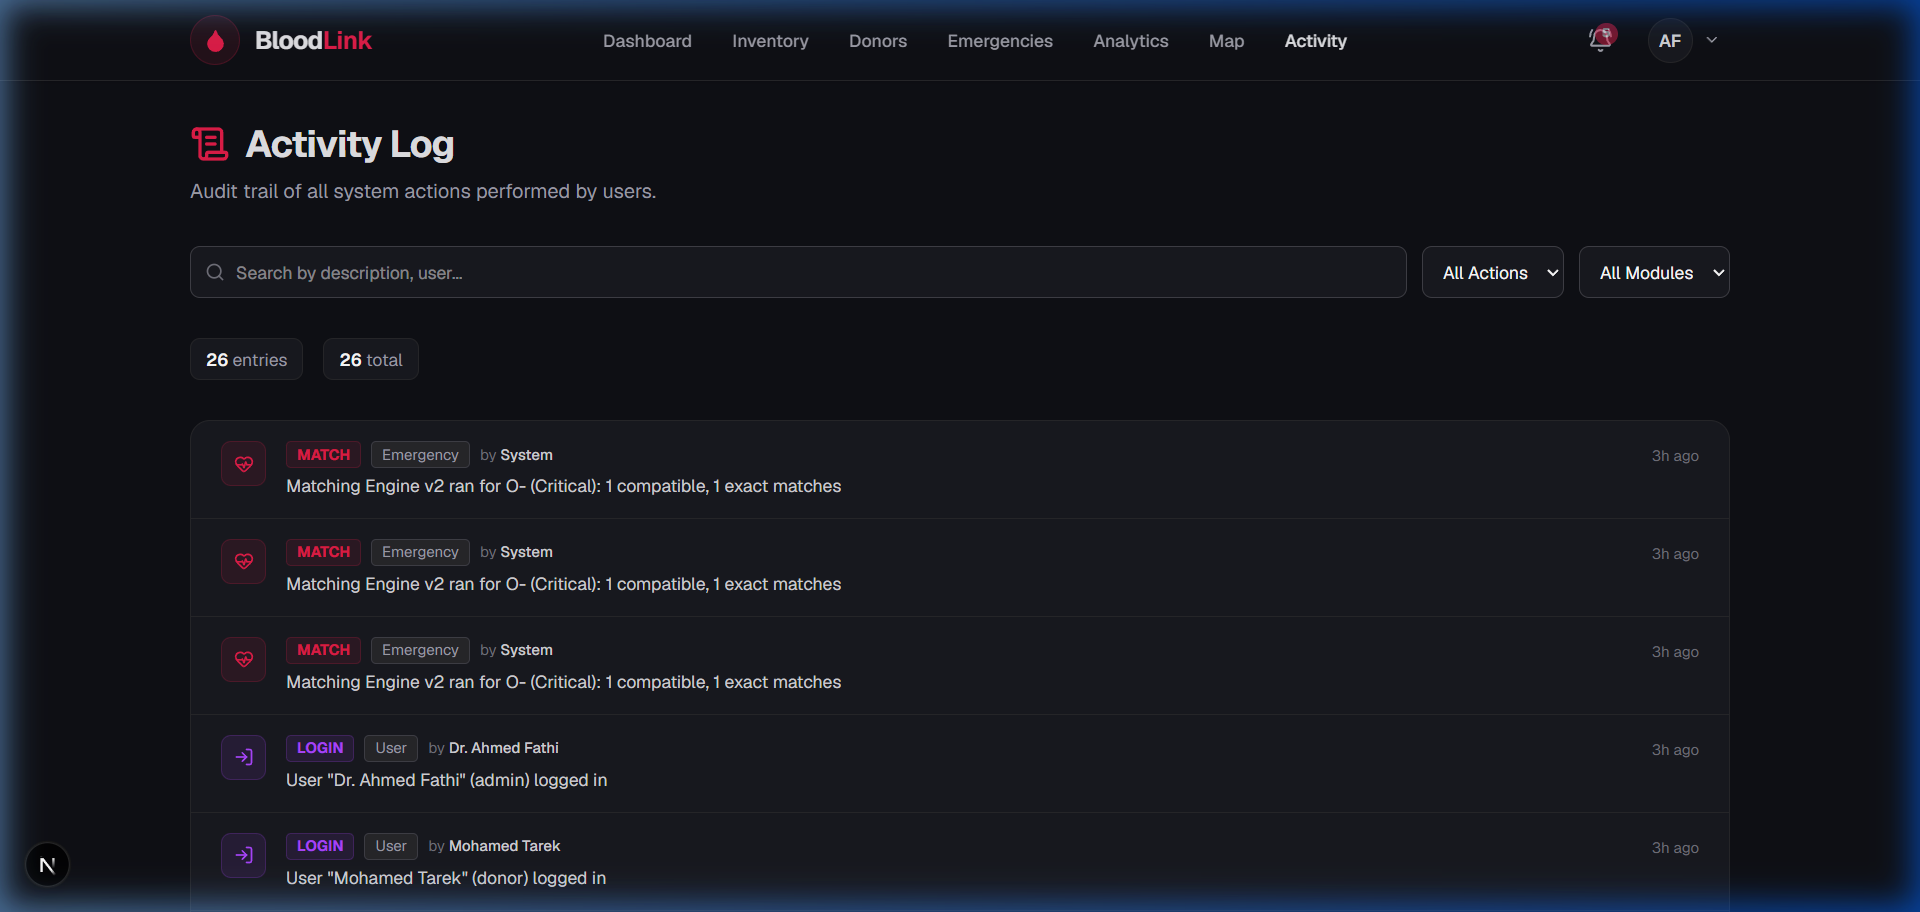
\includegraphics[width=\textwidth]{figures/activity.png}
    \caption{System Activity and Audit Log.}
\end{figure}

\section{Intelligent Matching Engine v2}
The cornerstone of BloodLink is its multi-factor donor matching algorithm. Rather than relying solely on blood compatibility, it scores and ranks donors based on a combination of factors, adapting its weights based on the emergency's urgency.

\subsection{Scoring Formula}
\begin{equation}
    Score = (Reliability \times W_r) + (Proximity \times W_p) + (ExactMatch \times W_e) - RecencyPenalty
\end{equation}

\subsection{Factors}
\begin{itemize}
    \item \textbf{Reliability (0-100):} Based on the donor's historical turnout rate.
    \item \textbf{Proximity (0-100):} Calculated using \textbf{Dijkstra's Algorithm} on a modeled road network graph of Cairo's 15 major districts, providing realistic driving distances rather than straight-line approximations. $Proximity = \max(0, 100 - (DistanceKm \times 2.5))$.
    \item \textbf{Exact Match Bonus (0 or 100):} Prioritizes exact blood type matches over merely compatible ones (e.g., O- for an O- patient is preferred over O- for an A+ patient if A+ is available).
    \item \textbf{Recency Penalty (0-25):} Enforces the WHO 56-day safety window. Donors who donated recently receive a proportional penalty, discouraging unsafe frequent donations.
\end{itemize}

\subsection{Urgency-Adaptive Weights}
The algorithm dynamically adjusts the weights ($W_r, W_p, W_e$) based on urgency:
\begin{table}[H]
\centering
\begin{tabular}{@{}lllll@{}}
\toprule
\textbf{Urgency} & \textbf{Reliability ($W_r$)} & \textbf{Proximity ($W_p$)} & \textbf{Exact Match ($W_e$)} & \textbf{Strategy} \\ \midrule
Critical & 35\% & 45\% & 20\% & Speed-first (closest reliable) \\
High & 45\% & 35\% & 20\% & Balanced \\
Medium & 55\% & 25\% & 20\% & Reliability-heavy \\
Low & 60\% & 20\% & 20\% & Quality-first (distance less critical) \\ \bottomrule
\end{tabular}
\end{table}

\section{Security and Authentication}
The platform ensures secure access through JWT-based authentication. Passwords are cryptographically hashed using bcrypt. The system enforces strict Role-Based Access Control (RBAC), distinguishing between Admins, Hospital Staff, Managers, and Donors, ensuring users only access authorized modules.

\begin{figure}[H]
    \centering
    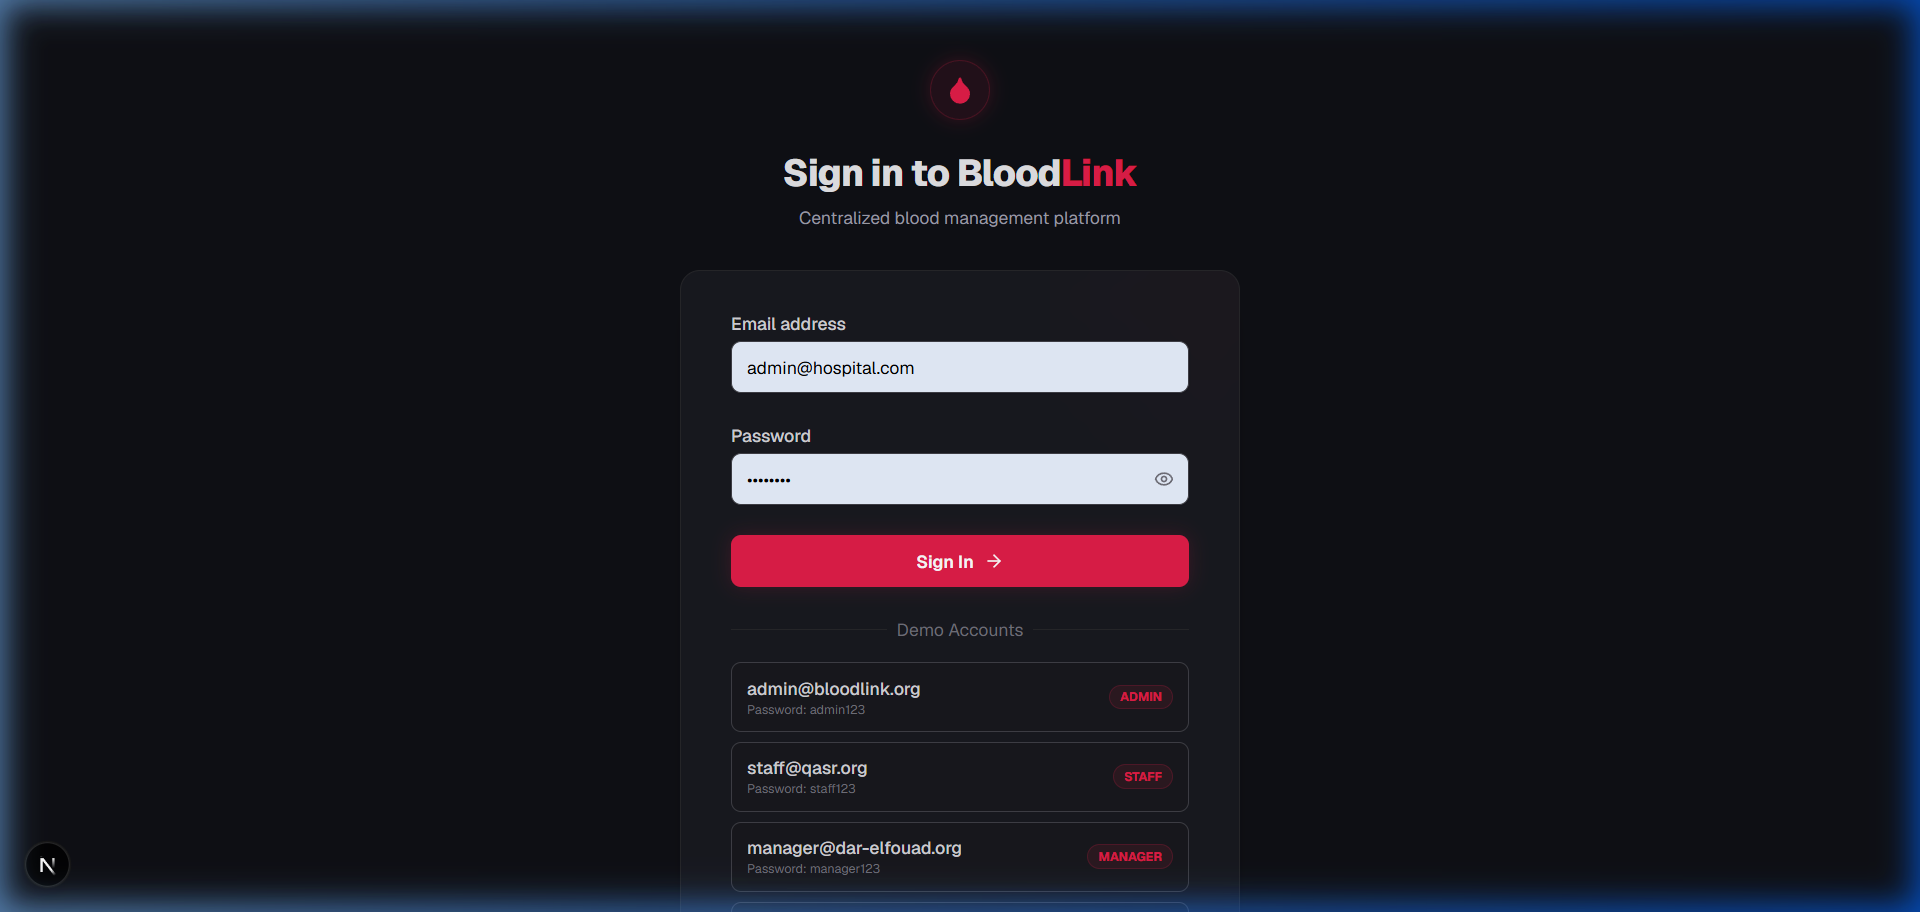
\includegraphics[width=\textwidth]{figures/login.png}
    \caption{Secure Login Portal with Demo Access.}
\end{figure}

\section{Conclusion}
BloodLink successfully transforms basic blood inventory management into a proactive, intelligent clinical system. By combining real-time tracking, an advanced geospatial matching algorithm, robust audit logging, and an intuitive dark-themed UI, the platform significantly reduces the time required to match critical patients with compatible, reliable donors.

\end{document}
